\documentclass[fleqn]{beamer}
\usepackage[english]{babel}

\usepackage{amsmath,amssymb}
\usepackage{graphicx}
\usepackage{hyperref}
\usepackage[absolute,overlay]{textpos}
  \setlength{\TPHorizModule}{1mm}
  \setlength{\TPVertModule}{1mm}

% vertical separator macro
\newcommand{\vsep}{
  \column{0.0\textwidth}
    \begin{tikzpicture}
      \draw[very thick,black!10] (0,0) -- (0,7.3);
    \end{tikzpicture}
}

% More space between lines in align
\setlength{\mathindent}{0pt}

% Beamer theme
\usetheme{ZMBZFMK}
\usefonttheme[onlysmall]{structurebold}
\mode<presentation>
\setbeamercovered{transparent=10}

% align spacing
\setlength{\jot}{0pt}

%\setbeamertemplate{navigation symbols}{}%remove navigation symbols

\title{DDoSGrid v2}
\subtitle{Integrating and Providing Visualizations for the European DDoS Clearing House}
\author{Jan von der Assen,\\ Muriel Franco, Bruno Rodrigues}
\institute[Master Thesis Midterm Presentation]{}
\date{\today}

\begin{document}

    \begin{frame}
      \titlepage
    \end{frame}
    
    \begin{frame}
      \frametitle{Table of Contents}
        Analysis and Improvement of Post-Mortem \\
        DDoS attack analysis tools.
        \begin{itemize}
          \item Motivation
          \item Related Work
          \item Requirements
          \item Implementation
          \item Demo
          \item Outlook
        \end{itemize}
           \begin{textblock}{20}(59,10)
          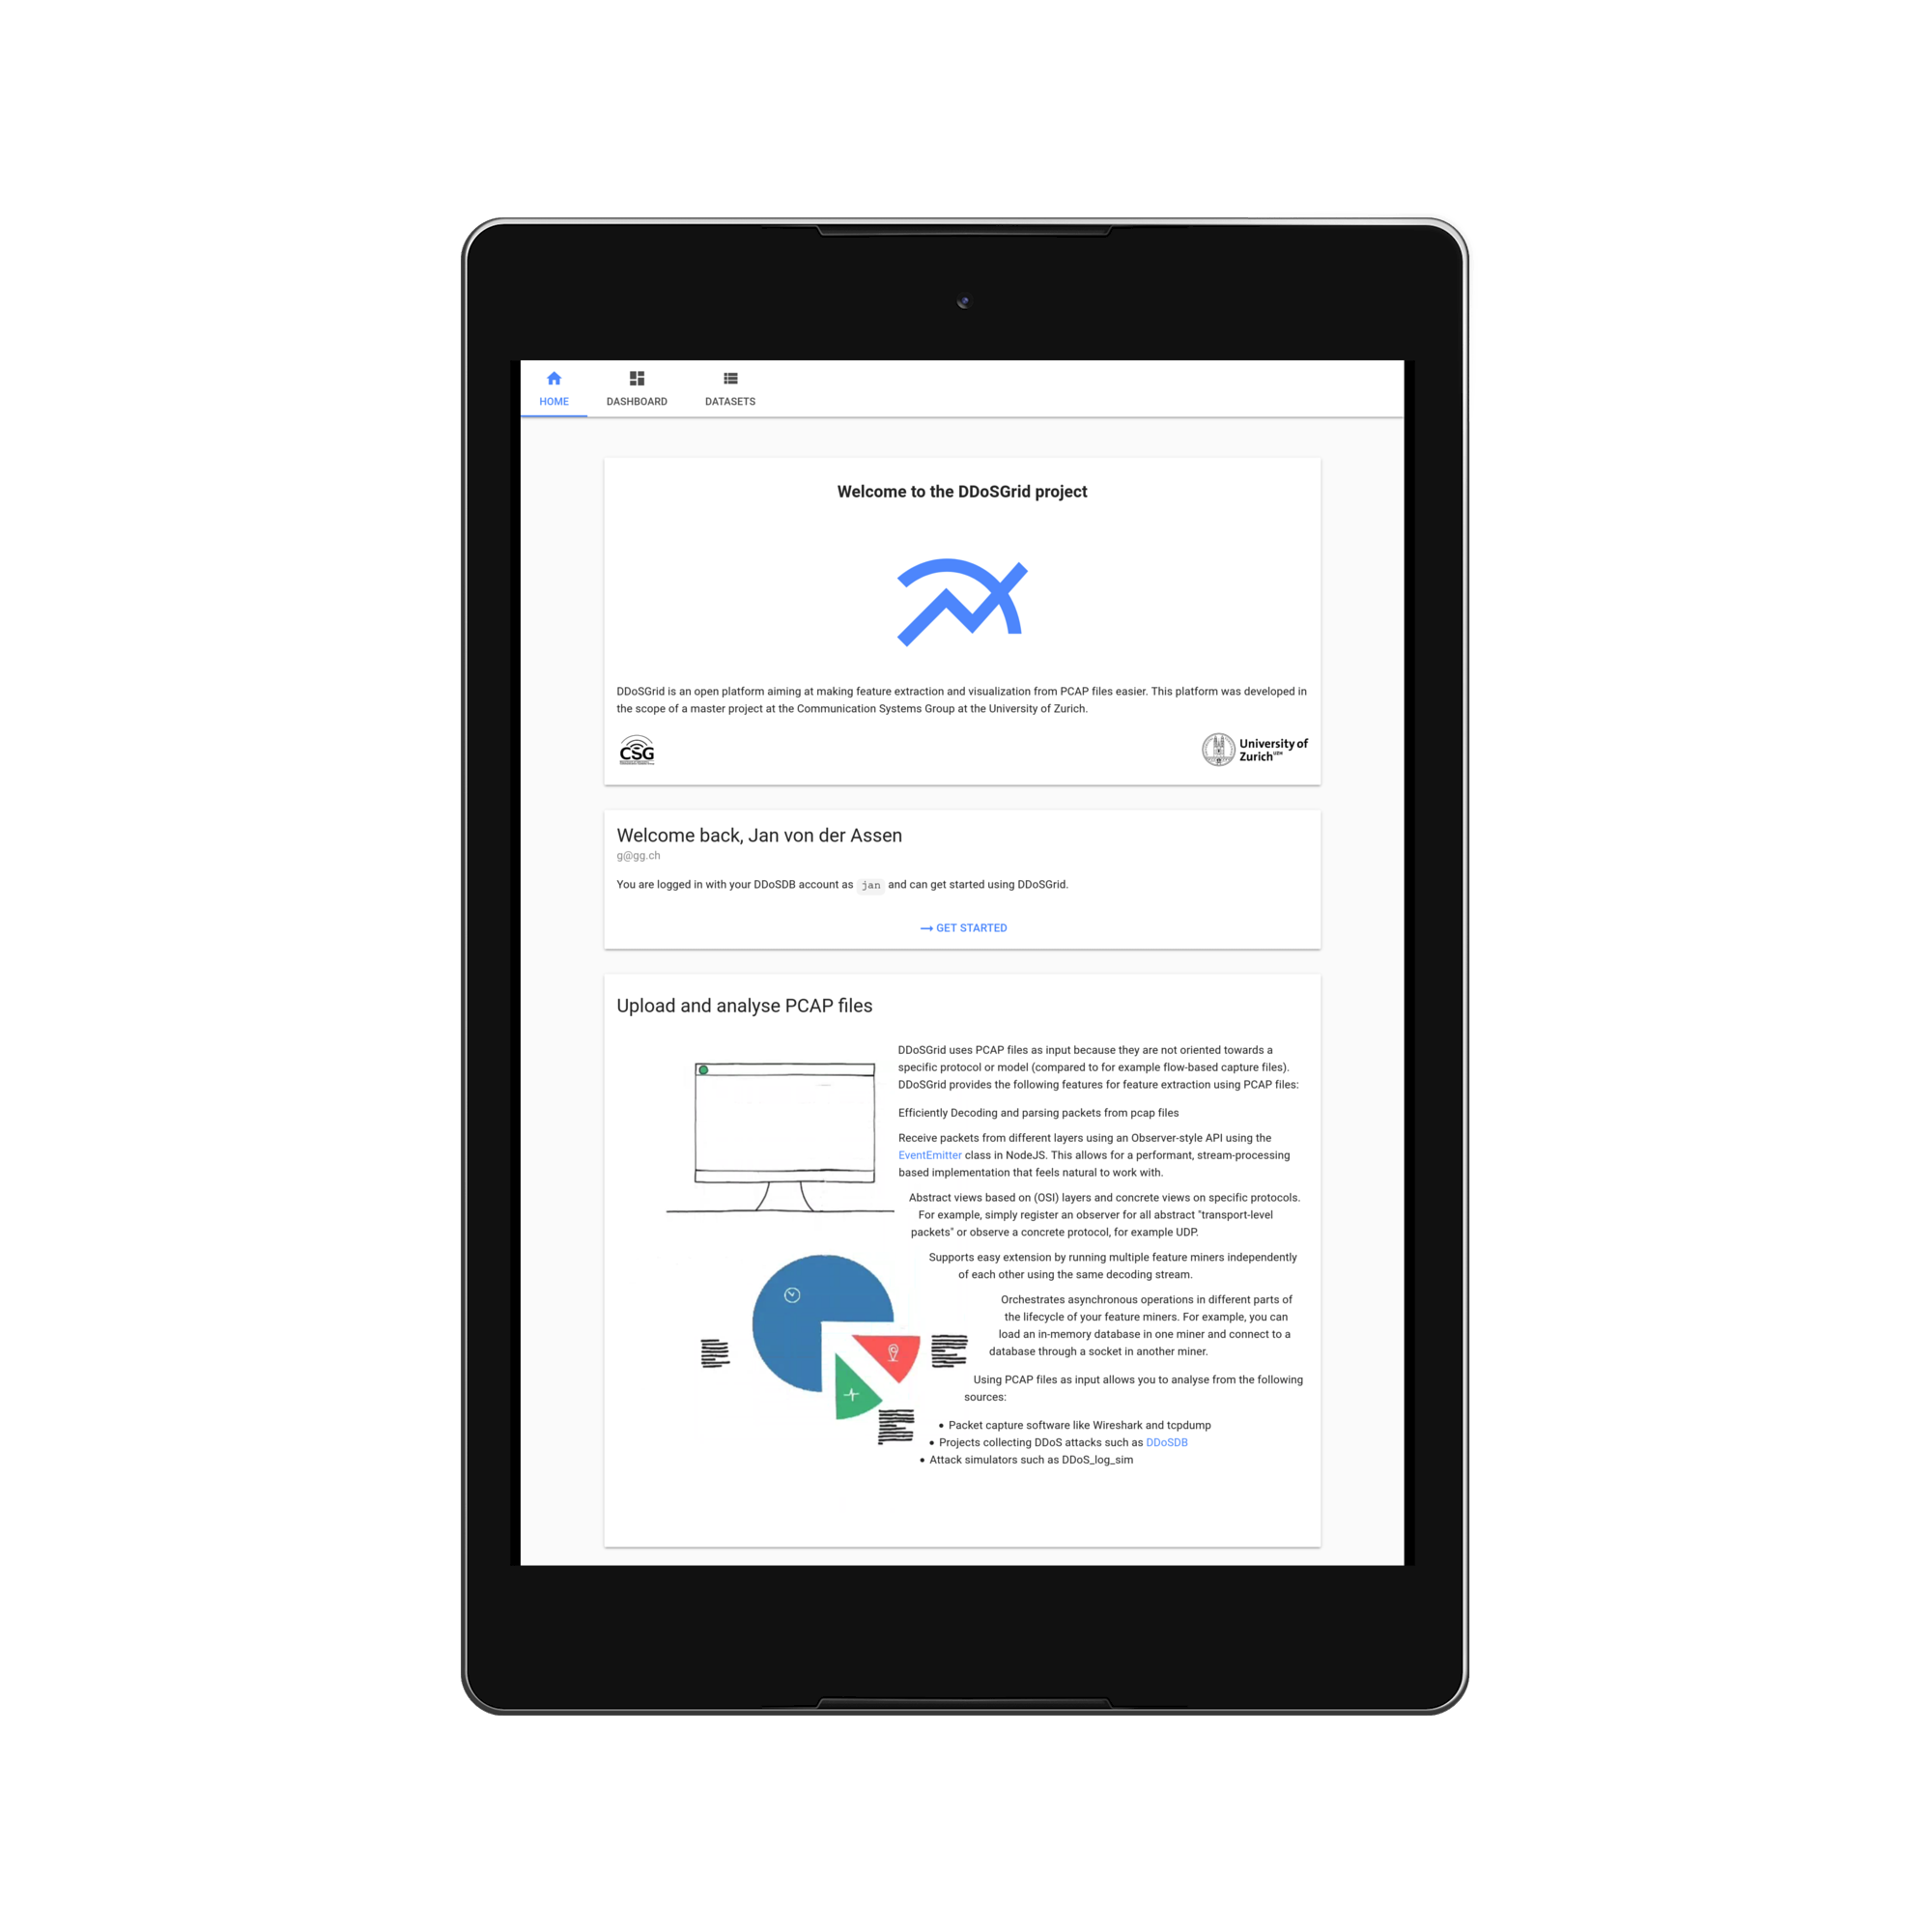
\includegraphics[scale=0.12]{images/google-nexus9-landscape.png}
          \end{textblock}
    \end{frame}
    
    \begin{frame}
      \frametitle{Motivation}
      \begin{columns}[T]
        \column{0.5\textwidth}
        DDoS Attacks
        \begin{itemize}
          \item Growing in Size
          \item Growing in Complexity
          \item Economic Impact
        \end{itemize}
        
        \column{0.5\textwidth}
          Example: Cloudflare (June 2020)
          \begin{itemize}
              \item Metrics
              \item Characteristics
              \item Assessment
          \end{itemize}
        
      \end{columns}
    \end{frame}
    
    \begin{frame}
      \frametitle{Related Work: Taxonomy}
          Post-Mortem (DDoS-) Analysis System
      \begin{itemize}
          \item Time\\
          \item Deployment Location\\
          \item Purpose
      \end{itemize}
    \end{frame}
    
    \begin{frame}
      \frametitle{Related Work: Literature Review}
      Reviewing existing work from literature and industry
      \begin{itemize}
          \item 17 Tools reviewed
          \item Properties elicited:
          \begin{itemize}
             \item Application
             \item Visual Transformation 
             \item Automation 
             \item Data Sources
             \item Implementation
          \end{itemize}
      \end{itemize}
    \end{frame}
    
    \begin{frame}
      \frametitle{Related Work: Literature Review}
      Findings:
      \begin{itemize}
          \item Limited Scalability \\
          \item Limited automation \rightarrow In-depth knowledge required\\
          \item "PCAP"-files de-facto data source\\
          \item Many Desktop-applications \\
          \item Focus on single aspect: Traffic Flow\\
          \begin{itemize}
              \item  DDoSDB: Sharing attack data\\
              \item DDoSGrid: Scalable Analysis- \& Visualization-Platform
          \end{itemize}
      \end{itemize}
    \end{frame}
    
    \begin{frame}
      \frametitle{Related Work: DDoSCH}
      Focus on promoting a \textbf{multi-lateral} view on DDoS attacks by providing a platform where \textbf{victims} are encouraged to \textbf{share} and \textbf{explore} attack data.\\
      \vfill
      DDoS Clearing House (DDoSCH) provides:
      \begin{itemize}
          \item DDoSDB: Web-application to explore attack (vict)
          \item Dissector: Anonymization, Fingerprint computation
          \item Converter: Transform insight into Firewall rules
      \end{itemize}
    \end{frame}
    
    \begin{frame}
      \frametitle{Related Work: DDoSGrid}
      Extracting and \textbf{visualizing} features of \textbf{DDoS attacks} using PCAP files. Focus on \textbf{efficiency}, \textbf{scalability} and \textbf{extensibility}.\\
      \vfill
      DDoSGrid consists of:
      \begin{itemize}
          \item Miner: CLI-tool to decode PCAP files and extract features
          \item RESTful web API: Interface, Orchestration, Metadata Storage
          \item Single-page Application: Visualization, Data Set Management
      \end{itemize}
    \end{frame}
    
    \begin{frame}
      \frametitle{Objectives}
      \begin{itemize}
          \item Integrating components from both projects to create a platform
          \item DDoSDB: Central component to store and explore data sets
          \item DDoSGrid: In-depth analysis, comparison and reporting on data sets from DDoSDB.
          
      \end{itemize}
    \end{frame}
    
    \begin{frame}
      \frametitle{Requirements}
      \begin{itemize}
          \item Literature Review: Find open aspects to contribute
          \begin{itemize}
              \item Integration to support exploration
              \item Powerful, Interactive Visualizations
              \item Scalable, Extensible Visual Transformation
              \item PCAP files as input
              \item High degree of automation
          \end{itemize}
          \item Architectural Analysis:
          \begin{itemize}
              \item Reuse authorization system (DDoSDB) - Privacy
              \item Provide stable interfaces (DDoSDB)
              \item Integrate and Automate components (dissector, converter)
              \item Provide User Interface - Hide technical details
          \end{itemize}
      \end{itemize}
    \end{frame}
    
    \begin{frame}
      \frametitle{Implementation Challenges}
      Three iterations that aim at a specific dimension of the overall solution:
      \begin{itemize}
          \item Models and Interfaces:
          \begin{itemize}
              \item Additional Authentication System
              \item Aligned Data Models
              \item Decoupled API
          \end{itemize}
          \item Automating the DDoSCH Life Cycle
          \item Usability
      \end{itemize}
      
    \end{frame}
    
    \begin{frame}
      \frametitle{Demo}
      \uncover<1>{
        \href{https://www.csg.uzh.ch/ddosgrid/}{ \nearrow   Authentication}
      }\\
      \uncover<2>{
        \href{https://www.csg.uzh.ch/ddosgrid/ddosdb/}{ \nearrow   Importing from DDoSDB}
      }\\
      \uncover<3>{
        \href{https://www.csg.uzh.ch/ddosgrid/datasets}{ \nearrow   Exporting to DDoSDB}
      }\\
    \end{frame}
    
    \begin{frame}
    \frametitle{Outlook}
      Evaluation:
      \begin{itemize}
          \item Performance Testing and Optimization
          \item Usability Evaluation
          \item Qualitative Evaluation
      \end{itemize}
    \end{frame}
    
    \begin{frame}
    \frametitle{Q\&A}
    \begin{center}
        \Large Question \& Answer
    \end{center}
    \end{frame}

\end{document}
